\section{Graph Networks}

\subsection{Message Passing Neural Networks}

Gilmer et al. describes Message Passing Neural Networks (MPNN) as a framework that generalizes at least eight models found in the literature ~\cite{Gilmer_2017}. The MPNN method describes a messaging and a readout phase on forward propagation.
	
The hidden nodes, hvt, are updated based on messages mvt+1, for a number of timesteps.

\begin{equation}
    \label{eqn:message}
    m^{t+1} = \sum_{w \in N(v)} M ^ {T} (h^t_v, h^t_w, e_{vw})
\end{equation}

\begin{equation}
    h^{t+1} = U_t(h^t_v, m^t_v)
\end{equation}

\begin{equation}
    \hat{y} = R (\{h^t_v | v \in G\})
\end{equation}

\begin{itemize}

    \item The message function, $M^{t}$, plays the role of the GN’s $\phi ^ e$, but does not take $u$ as input,
    
    \item Element wise summation is used for the GN’s $\rho ^ {e \rightarrow v}$,
    
    \item The update function, $U_t$, plays the role of the GN’s $\phi ^ v$
    
    \item The readout function, $R$, plays the role of the GN’s $\phi ^ u$, but does not take $u$ or $E'$ as input, and thus an analog to the GN’s $\rho ^ {e \rightarrow u}$ is not required;
    
    \item $d_{\text{master}}$ serves a roughly similar purpose to the GN’s $u$, but is defined as an extra node connected to all others, and thus does not influence the edge and global updates directly. It can then be represented in the GN’s $V$.

\end{itemize}

\begin{figure}[!htb]
    \centering
    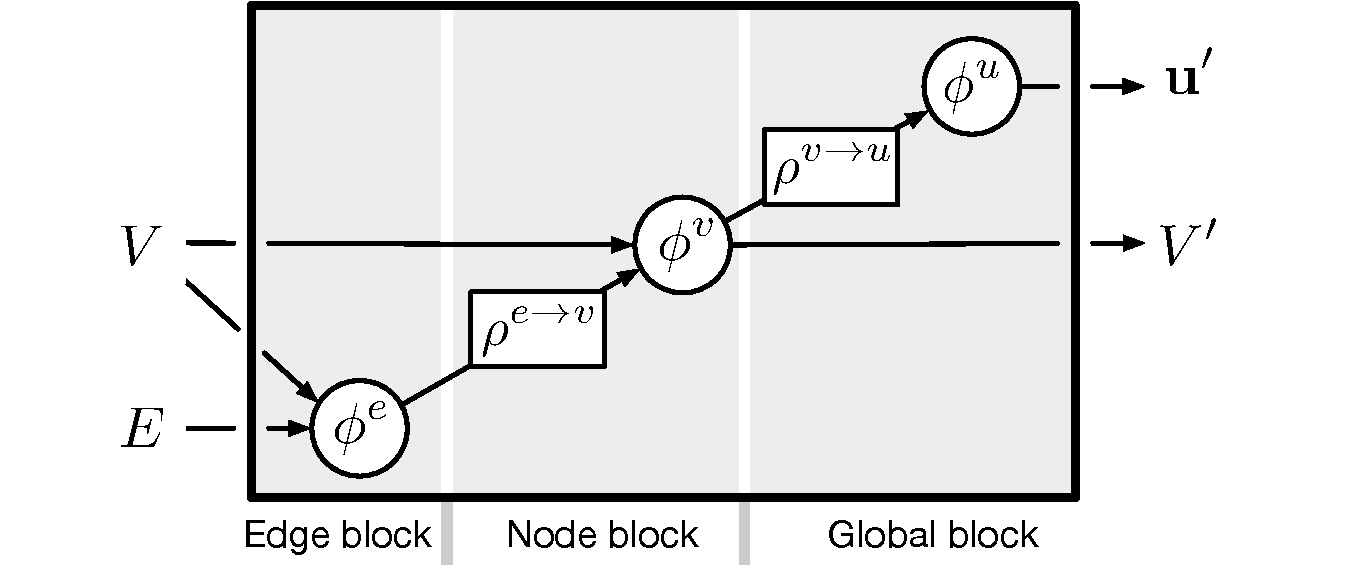
\includegraphics[height=3.0cm]{fig/content/graph_nets/blocks/mpnn.pdf}
    \caption{The forward pass phases of the Message Passing block elicited above ~\cite{Battaglia_2018}.}
\end{figure}



\subsection{Non Local Neural Networks}

Both recurrent and convolutional operations are building blocks that process one local neighborhood at a time. On the other extreme, fully connected layers have those relations encoded in the learned weights, therefore the relationship between the points is not a direct function of the input layer. 

Non Local Neural Networks (NLNN), ~\cite{Wang_2018} presents a mid-term building blocks for capturing long-range dependencies.

In it, the forward pass is computed by repeatedly applying a weighted sum of a function of the previous step, but in this case part of the weight is a similarity measure between the node being calculated and the node being summed over.

\begin{equation}
    h^{t+1}_v = 
    \cfrac{1}{C(h^t)} 
    \cdot \sum_{\forall u \in V} {
        f(h^t_v,h^t_u) \cdot g(h^t_u)
    }
\end{equation}

\begin{figure}[!htb]
    \centering
    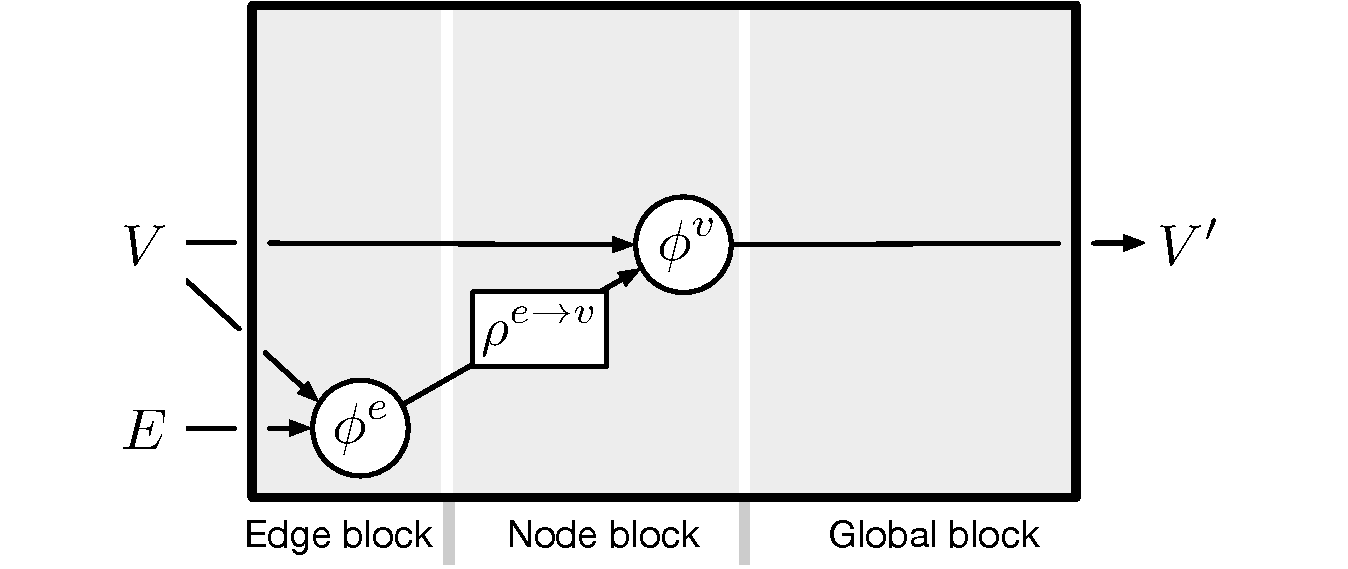
\includegraphics[height=3.0cm]{fig/content/graph_nets/blocks/nlnn.pdf}
    \caption{The forward pass phases of the Non Local Neural Network block ~\cite{Battaglia_2018}.}
\end{figure}

\subsection{Graph Independent}

The Graph Independent module applies models to the graph elements independently, that is, the models are applied to each element of the graph (nodes, edges and globals) in parallel and independently of the other elements.

\begin{figure}[!htb]
    \centering
    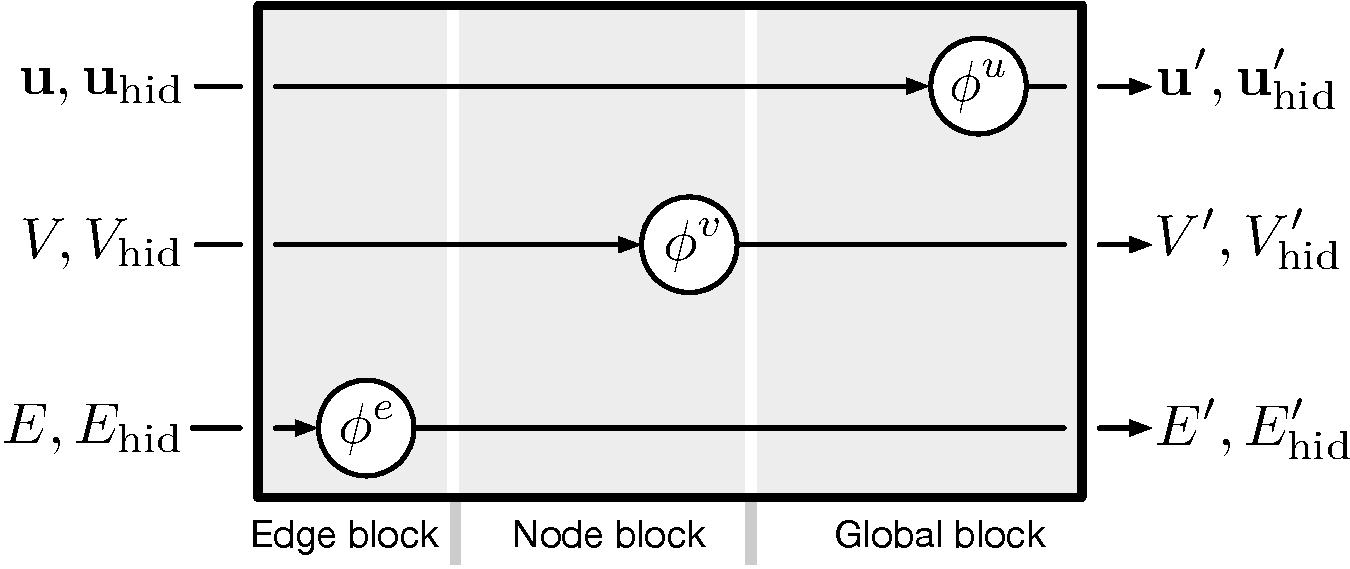
\includegraphics[height=3.0cm]{fig/content/graph_nets/blocks/independent.pdf}
    \caption{The forward pass phases of the Graph Independent block ~\cite{Battaglia_2018}.}
\end{figure}

\subsection{Graph Nets}

The Graph Networks (GN) framework generalizes and extends various graph neural network approaches, such as MPNN and NLNN (Non Local Neural Networks) ~\cite{Battaglia_2018}. A Graph Net is composed of blocks which operate a sequence of steps according to its configuration. One possible configuration, a full GN block (a), predicts node, edge, and global features based on its incoming nodes, edges, and global features.

Graph Nets framework encompasses flexible representations, configurable in-block structure and composable multi-block architectures ~\cite{Battaglia_2018}. This is shown in the example block arrangements in \ref{fig:graph_nets_flexibility} In each block, $\phi$ (phi) functions may be applied to incoming attributes and $\rho$ functions to aggregate them, generating new, updated output values (shown as either $u'$, $V'$ or $E'$).

\begin{figure}[!htb]
    \centering
    \subfigure[Full block]{
        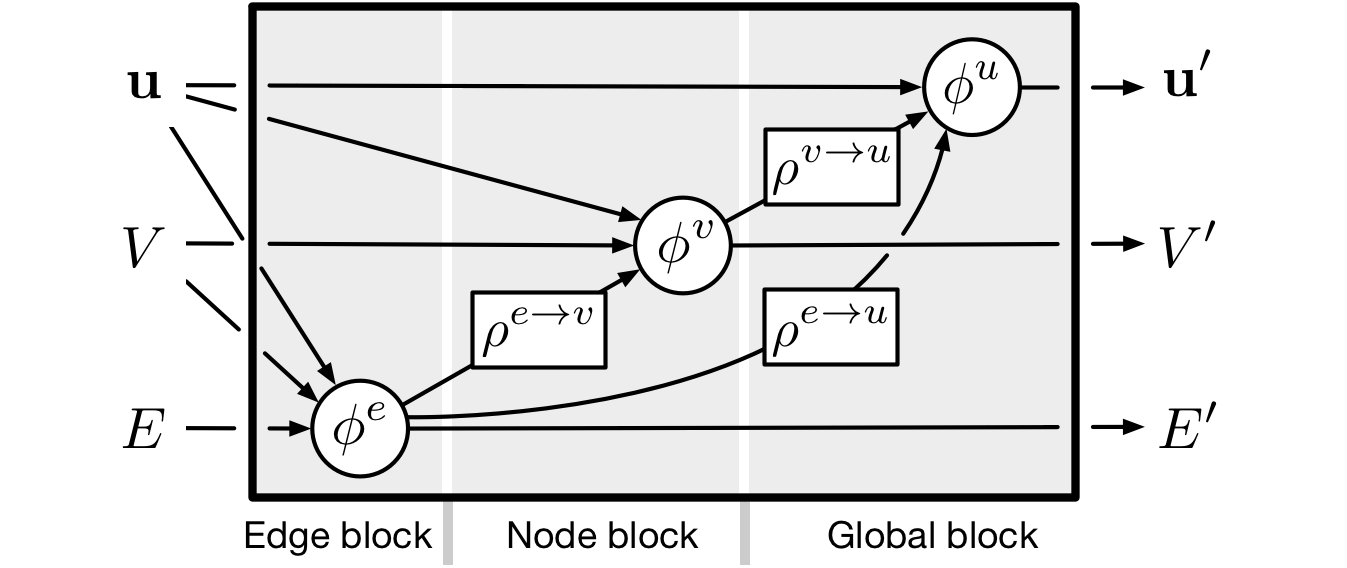
\includegraphics[width=.45\linewidth]{fig/content/graph_nets/blocks/full.png}
    }
    \subfigure[Independent block]{
        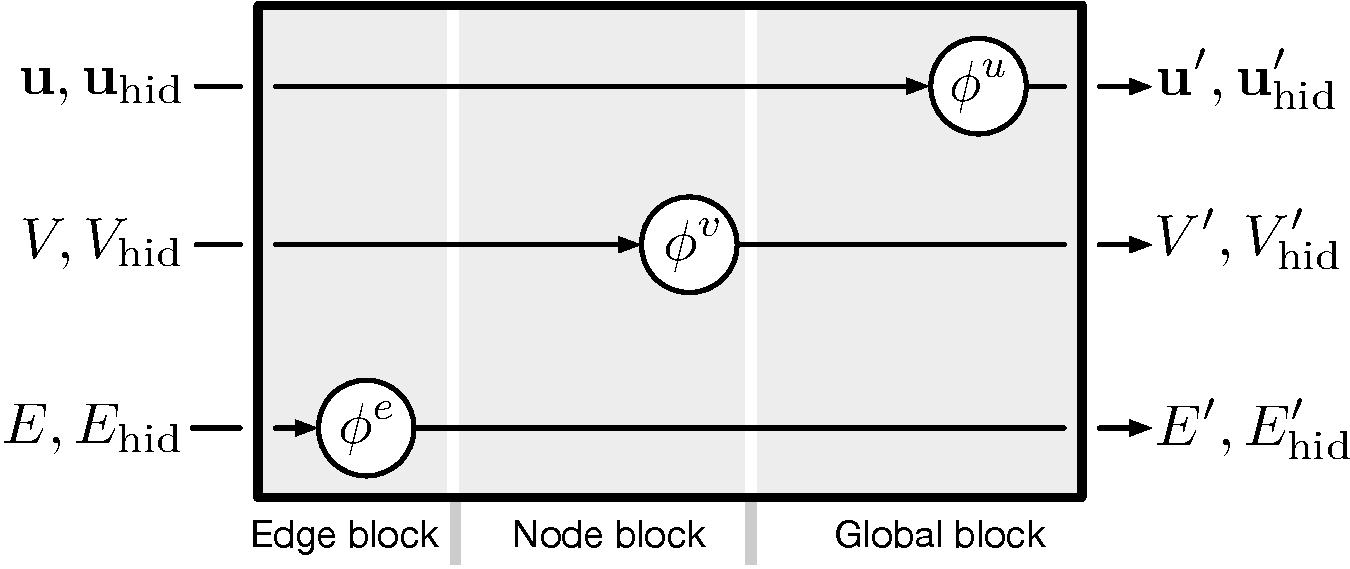
\includegraphics[width=.45\linewidth]{fig/content/graph_nets/blocks/independent.pdf}
    }
    \subfigure[Message-passing block]{
        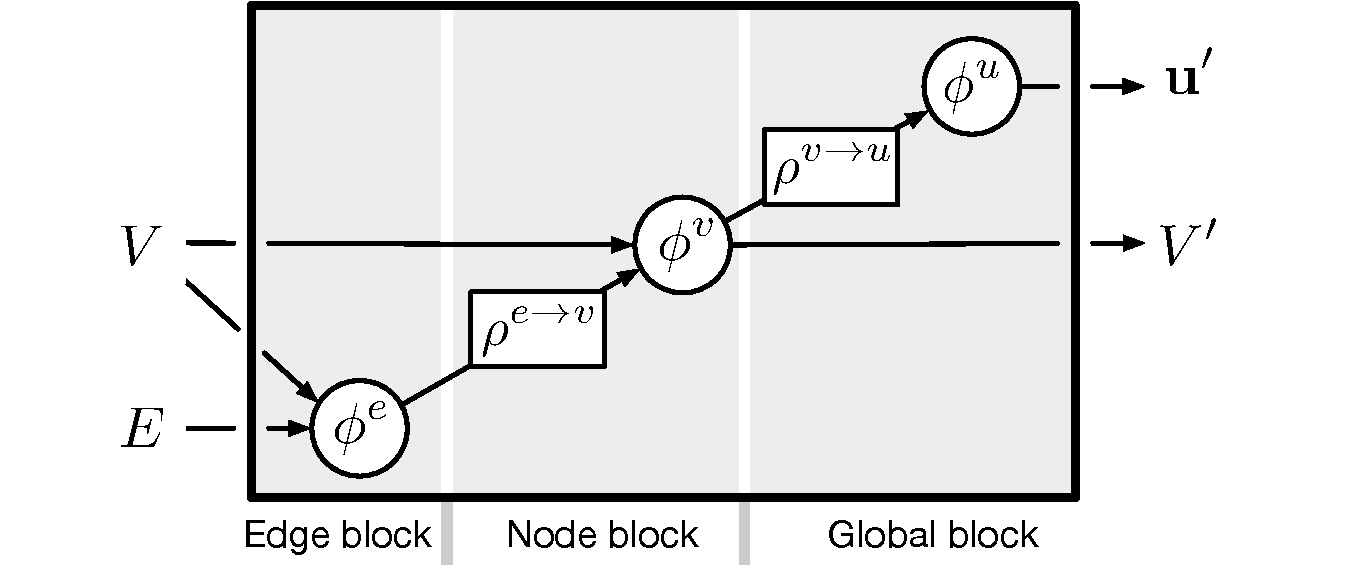
\includegraphics[width=.45\linewidth]{fig/content/graph_nets/blocks/mpnn.pdf}
    }
    \subfigure[Non Local block]{
        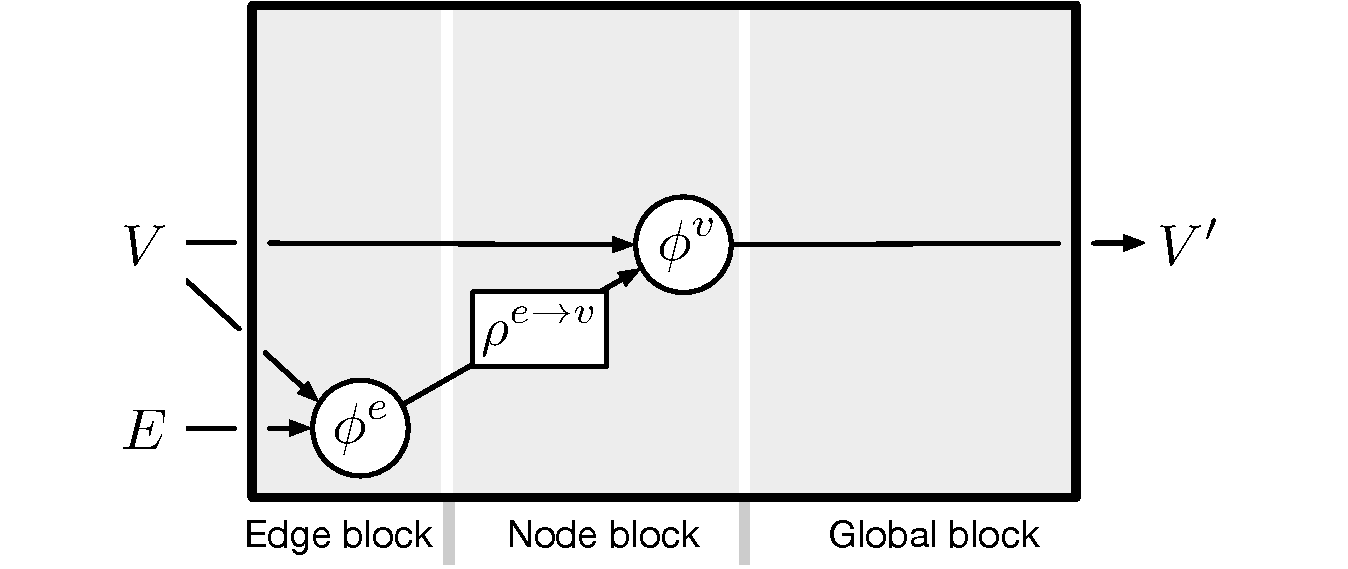
\includegraphics[width=.45\linewidth]{fig/content/graph_nets/blocks/nlnn.pdf}
    }
    
    \caption{Graph Nets internal block configurations ~\cite{Battaglia_2018}}
    
    \label{fig:graph_nets_flexibility}
\end{figure}




\section{Analyzed Problems}


\subsection{State Prediction of a Spring-mass System}

This problem explores a computational simulation derived from an actual physics experiment. Given a set of masses connected one another by springs, with two of them fixed, e.g. pinned to a wall, the problem is to predict the next state of the masses after  some noise was applied.

The state of the masses is defined as a 2-D position and velocity. The system always starts from rest position, with all masses in the same vertical position and zero velocity in the two dimensions. They also start with the same distance apart from one another.

A computational simulation of this system was carried out by Battaglia et al. (2016)'s "interaction networks" ~\cite{Bataglia_2016} using deep learning and more recently in ~\cite{Battaglia_2018}. In the simulation, a random dataset is generated by initializing nodes with fixed spacing among them, and then applying noise on every timestep.

In the system, masses are translated into nodes and springs into edges. This produces a graph where each non-fixed node has two adjacent neighbors. The vertex feature vector is composed by the tuple $(x, y, v_x, v_y, \text{fixed})$, where $x$, $y$ denote position, $v_x$, $v_y$ denote velocity and fixed denotes whether a mass is fixed.

The edges’ feature vector is composed by the springs’ rest distance and their constants. The global feature vector is composed solely by the gravitational acceleration, which is -10m/s².

The model generates a trajectory by applying noise at each iteration of the simulation. By the end, a graphs dataset is ready to be input into the neural network. Training data examples have 5 to 8 masses, while test data have 4 to 9 masses.

\begin{figure}[!htb]
    \centering
    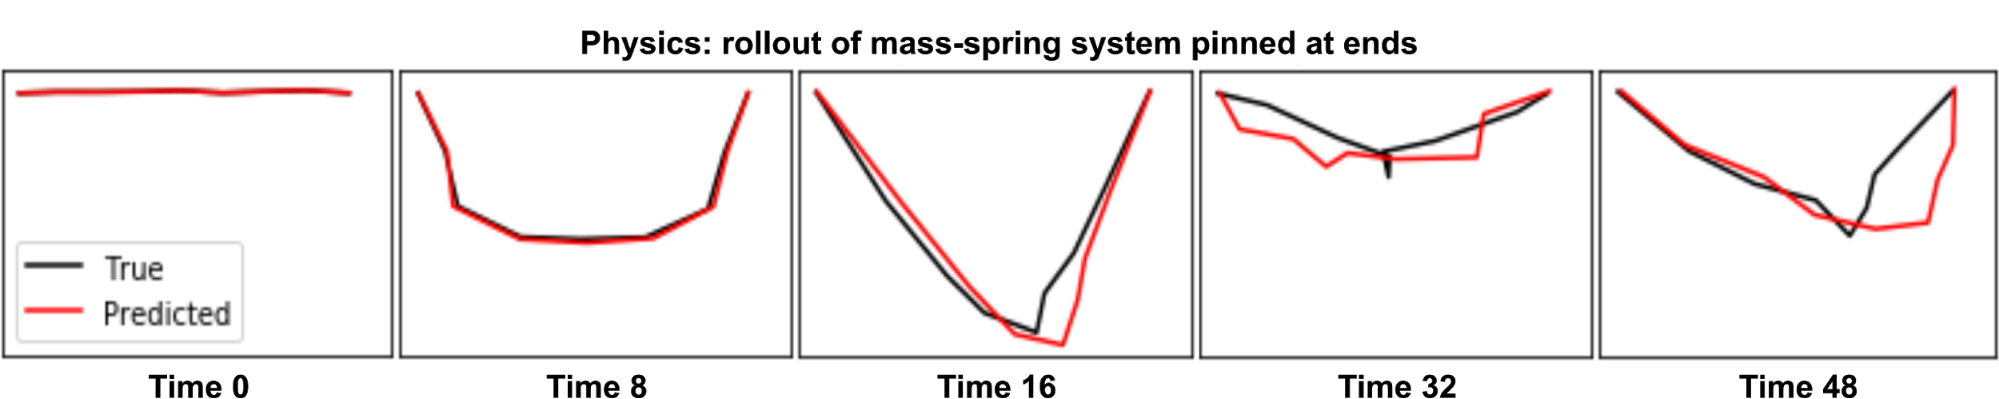
\includegraphics[height=3.0cm]{fig/content/analysed_problems/physics/tragectory.png}
    \caption{Predicted and true values from states along a spring-mass trajectory ~\cite{Battaglia_2018}.}
\end{figure}


\subsection{Shortest Paths}

The experiment creates random graphs, and trains a graph network to label the nodes and edges on the shortest path between any two nodes. Over a sequence of message-passing steps, the model refines its prediction of the shortest path.

\begin{figure}[!htb]
    \centering
    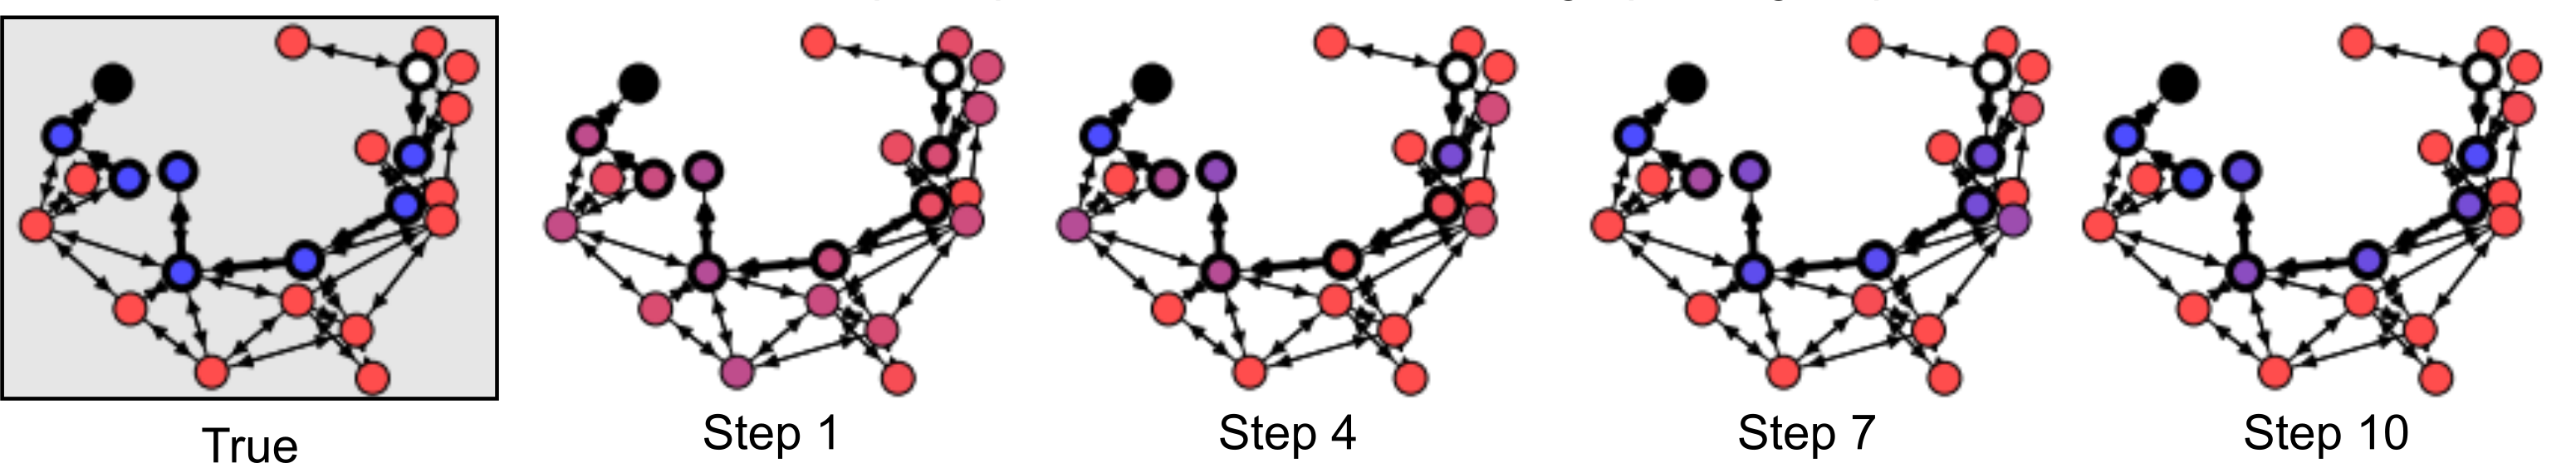
\includegraphics[height=3.0cm]{fig/content/analysed_problems/shortest_paths/steps.png}
    \caption{Prediction at each message-passing step for shortest path problem ~\cite{Battaglia_2018}.}
\end{figure}


\subsection{Regions Separation}

The problem here is the classification of pixels of an input image, given its similarities with its neighbors. 

At first glance, this problem might not seen related with a graph to graph problem, but we can make a reduction of this problem to one of finding a set of independent connected components that represent each of the different classes of pixels. 

So the input is transformed into a graph network with one vertex for each pixel and a link of two vertices if the corresponding pixels are neighbors.

The output can be transformed simply by partitioning the graph with a Depth First Search (DFS) or using the vertex class feature that the reduced problem must also provide.

The problem that we explored is the reduced one: Given the graph network described and exemplified below, with features indicating color and position in each vertex, produce the graph with vertices of different regions in different connected components and with features indicating in what region the vertex is. Since the set of edges in the solution is always a subset of the edges in the input, we used an edge feature to indicate if the corresponding edge is part of the solution.

\begin{figure}[!htb]
    \centering
    
    \subfigure[Input image and associated graph]{
        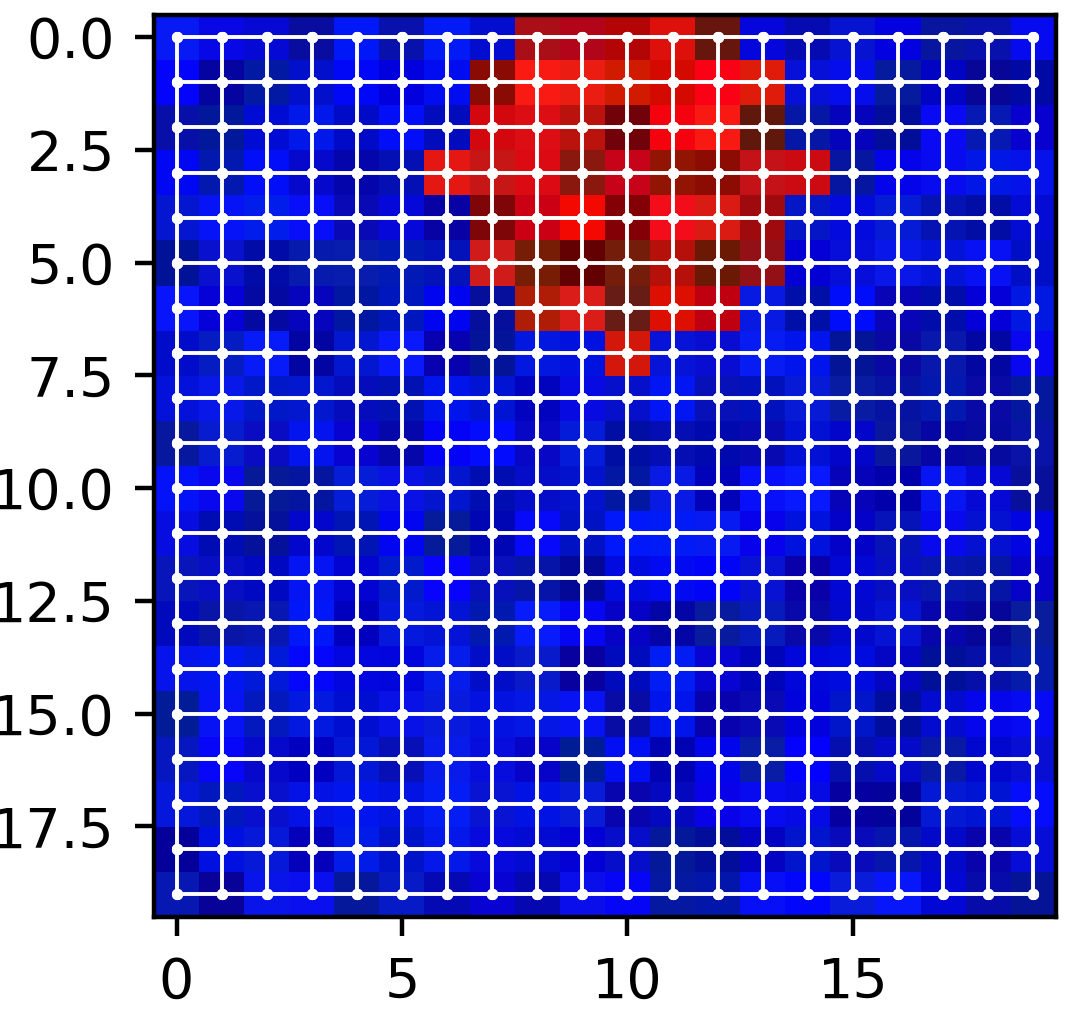
\includegraphics[width=.45\linewidth]{fig/content/analysed_problems/shapes/input.png}
    }
    \subfigure[Expected image and associated graph]{
        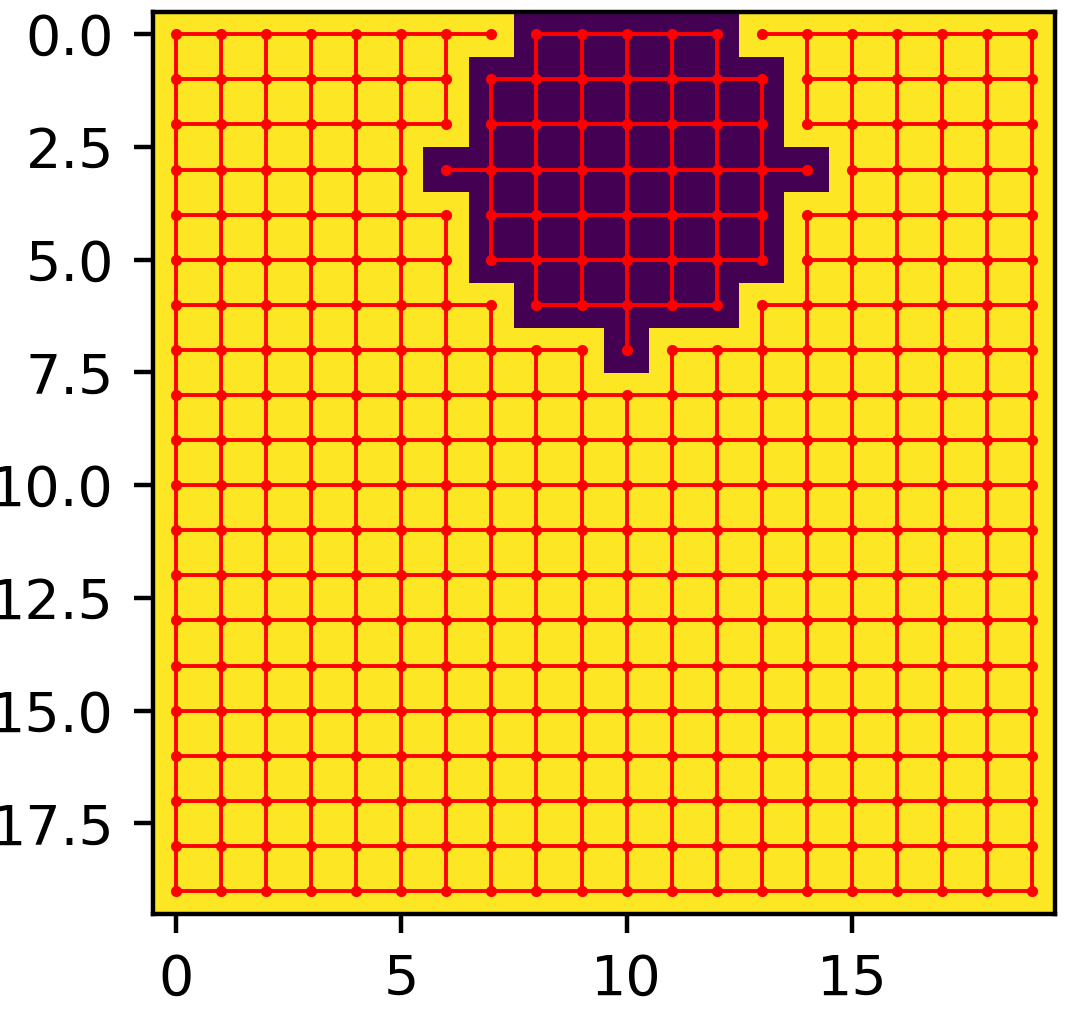
\includegraphics[width=.45\linewidth]{fig/content/analysed_problems/shapes/expected.png}
    }
    
    \caption{Visualization of an entry of the dataset used for the Region Separation problem}
    
    \label{fig:regions_separation_dataset_visualization}
\end{figure}




\section{Methodology}


\subsection{The Model}


\subsection{Physics Experiments}


\subsection{Shortest Paths Experiments}


\subsection{Regions Separation Experiments}



\section{Results and Discussion}


\subsection{Experiments A - Physics}

\subsubsection {Permutation of test sets}

\subsubsection {Permutation of training sets}


\subsection{Experiments B - Shortest Paths}

\subsubsection {Permutation of the testing set}

\subsubsection {Permutation of the training and testing sets}


\subsection{Experiments C - Regions Separation}

\subsubsection {Permutation of test sets}

\subsubsection {Permutation of training sets}